\justifying
\section{Introduction}
According to Aristotle, in order to explain the world and objects around us we need to recognize four causes: i) the matter determined by the material of the object; ii) the form determined by the shape of the object; iii) the agent determined by the transformation of the object; and iv) the end determined by the purpose of the object.\cite{ARI} Although this knowledge was professed more than 2000 years ago, there is analogism with modern science. In particular, in materials science and/or nanotechnology when we describe an object, we tend to refer to those four causes: i) the matter is the chemistry of the material; ii) the form is the morphology of the material; iii) the agent is the process through which a material is modified; and iv) the end is the functionality of the material.\\
For new nanomaterials, it is fundamental to well-define their morphology and chemistry, since different chemo-morphological combinations will lead to diverse surface and quantum size phenomena. For this reason, nanomaterials such as carbon nanotubes (CNTs) are undergoing a standardization process, which tabulates all relevant CNTs properties and standard protocols for characterization.\cite{IEC} A similar standardization process will be necessary for graphene oxide (GO), which can be thought as a single layer carbon sheet (\textit{i.e.}, graphene) decorated with oxygen functionalities, involving both basal-plane and edge-site chemical modification of graphene during oxidation and exfoliation. The standardization process can be included in the current effort to introduce a rational naming system for the two-dimensional carbon form.\cite{bianco2013all}\\
GO has recently gained interest among academic researchers and industries. From the academic sector, the number of citations per year of scientific work whose title includes ''graphene oxide'' has increased by almost one order of magnitude (from $\approx900$ to $\approx7000$, Fig.~\ref{Fig1_pap3} in four years ($2011-2015$)\cite{WEB}. From the industrial sector, the GO manufacturing capacity has increased by a factor of five over roughly three years, with a current yearly production capacity of $\approx1000$ tons/year.\cite{zurutuza2014challenges,peplow2015graphene} Moreover, the number of annual patents filed whose title contains ''graphene oxide'' has increased by an order of magnitude in four years ($2011-2015$).

\begin{figure}[h!]
  \centering
  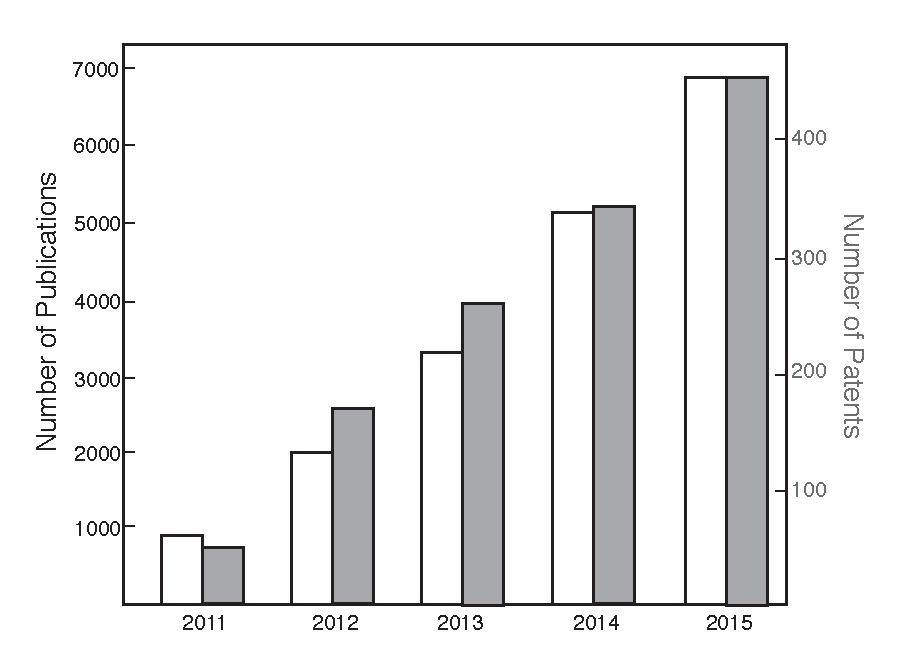
\includegraphics[width=5in]{paper3/Fig1.pdf}
  \caption{\textbf{GO trends.} Number of publications (white) and number of patents filed (gray), with a title that contains ''graphene oxide'', between 2011 and 2015.}
  \label{Fig1_pap3}
\end{figure}

The drive behind this increased interest is two-fold. First, the GO price per gram is about six orders of magnitude lower than pristine graphene, which opens different markets such as industrial applications. The price of GO is also steadily declining due to the development of scalable fabrication systems with current reactor capacity $>100$ tons/year, which leads companies to predict a GO price as low as a few cents per gram in the next five years. These factors also raise the interest of investors and producers who want to place themselves in the market before an explosion of growth dictated by successful demonstration of applications; similar to what recently happened with quantum dots, which found their
market in the display industry.\cite{shirasaki2013emergence}\\
Second, GO displays unique properties such as near-atomic
thickness,\cite{novoselov2012} the presence of oxy-groups allowing for rapid functionalization,\cite{Dreyer2010} scalable synthesis processes,\cite{park2009chemical} and the possibility of controlled deposition of nanothin films on a variety of substrates using solution-based casting techniques (\textit{e.g.}, vacuum filtration,\cite{Han2013,nair2012unimpeded} spin coating ,\cite{shen2016subnanometer,wang2016dramatic} layer-by-layer,\cite{silverberg2017controlling} or doctor blade printing\cite{akbari2016large}). More importantly, the versatility and the possibility of tuning the primary GO properties (flake size and quantity of oxy-functionalities) led researchers to propose the use of GO in several fields such as energy storage \cite{ogata2017all,yoo2011ultrathin} separation processes ,\cite{wang2016dramatic,mi2014graphene,fathizadeh2017graphene} and drug delivery,\cite{liu2013graphene,wang2014reduced} just to mention a few (readers can refer to exhaustive literature reviews of GO applications).\cite{georgakilas2016noncovalent} In each specific application, the GO properties have been selected \textit{ad hoc} to serve at best the functionality of the device in which GO is implemented. For example, in transparent conducting films, large-dimension and slightly-oxidized GO flakes are selected in order to enhance electron transport.\cite{mattevi2009evolution,eda2008large}  Although slightly-oxidized GO flakes are also preferred for supercapacitor applications, recent studies explored the possibility of exploiting surface GO oxy-functionalities to increase device pseudo-capacitance via red-ox reactions.\cite{jana2015non} GO morphology is paramount for the enhancement of mechanical properties; for instance, large size GO flakes are preferred to maximize fiber reinforcement.\cite{cano2013improving} In membrane technology for water treatment, the number of oxy-functionalities and GO dimensions can be tailored accordingly to the contaminant of interest and desired permeability;\cite{mi2014graphene} thus, the rational modification of the GO nanoproperties will allow controlled tuning of the permeability-selectivity trade-off.\\
In order to enable successful commercialization and industrial application of GO, it is paramount that researchers and industries have a common understanding of GO nomenclature and properties, which can have a large impact on the application of interest, vida supra. However, from our experience, studies in the literature, and discussions with academics and GO producers, GO properties are extremely wide-ranging, source-dependent, and, in some of the cases, are not even mentioned. In particular, the synthesis process plays a major role in determining GO properties. GO can be synthesized from 3D graphite flakes via the Hummers' method,\cite{Hummers1958} which represents an evolution of two previous chemical exfoliation methods (Brodie and Staudenmaier).\cite{Dreyer2010} As it has been recently shown, even small tuning of the synthesis process (\textit{e.g.}, time and/or temperature of the oxidation process) can lead to significantly different GO properties.\cite{chang2016guidelines} One clear example illustrating how poor GO characterization can lead to confusion in the research field is the recent controversy on the water transport in GO laminates. On one hand, studies have reported fast water transport (FWT) in GO possibly due to the low wall friction experienced by water when traveling through regions of 2D pristine graphene capillaries;\cite{nair2012unimpeded,abraham2017tunable} this is similar to FWT through 1D CNT due to a linear water- water dipole alignment parallel to the CNTs axis offering the lowest water-CNTs interaction.\cite{zuo2009transport} On the other hand, surface friction might occur when water travels through GO nanochannels depending on the amount and type of GO basal plane oxy-groups.\cite{willcox2017molecular,montessori2017extended,dai2016water,chen2017molecular} The origin of this controversy most likely arises from the difference in nanoproperties of the compared GO materials. Thus, it is fundamental that GO properties are well characterized when proposing theories and/or in order to enable a fair comparison between research results.\\
This work here aims to initiate the GO standardization process offering: i) high-throughput and lab-accessible GO characterization protocols and ii) a GO classification according to properties based on a clustering algorithm. The classification is similar to what has been done for bulk materials, which are divided into sub-categories (\textit{e.g.}, high-density polymer versus low-density polymer). The standardized characterization protocols are then validated by six GO samples collected from different producers across two continents. Investigation of GO-based applications utilizing material from different producers is used to highlight the effect of the nanomaterial properties on the macroscopic performance of a device.
\section{Methods}
\subsection{Materials}
GO was acquired from six different producers across two continents. Depending on the producer, the GO was either received in powder form or in an aqueous solution. All the samples were then diluted in water to the same concentration (0.05 wt\%) and then subjected to the specific pretreatment required by the producer; possible pretreatments include sonication with a \textit{Branson} sonicator ($V=1.9$ L, $max power=480$ W, and $f=420$ kHz) and pH adjustment with NaOH. The polyvinylidene difluoride (PVDF) membrane used as the support for the vacuum filtered GO thin film was purchased from \textit{Sterlitech} (\textit{TriSep YMTM103001}). The PVDF membrane was cleaned by ultrasonication in IPA for 5 min, then in DI for 5 min, and kept in IPA prior to use. Escherichia Coli B (\textit{E. coli}) CAROLINA\textsuperscript{TM} 124300 (\textit{Carolina Biological Supply Company}) was utilized as a model bacterium to evaluate the bacterial deposition on the GO membranes. \textit{BD Bacto\textsuperscript{TM}} tryptic soy broth (TSB), tryptic soy agar (TSA), NaCl (reagent grade), and ethanol (EtOH; laboratory grade) were purchased from \textit{VWR International}. Formaldehyde (35\% in water) was purchased from \textit{Sigma-Aldrich}. Deionized (DI) water ($>18$ M$\Omega$) was produced by a \textit{Nanopure Infinity} ultrapure water system (Barnstead/Thermolyne) and was used to prepare solutions and rinse containers. Methylene blue hydrate ($>95$\%) was purchased from \textit{Sigma-Aldrich} and selected to evaluate the adsorption capacity of the different types of GO samples examined.

\subsection{Structure and Morphology Characterization}

\textbf{Scanning electron microscopy (SEM):} A \textit{Zeiss ULTRA} Field Emission Scanning Electron Microscope with an In-lens secondary electron detector was used to characterize the GO morphology. The working distance, acceleration voltage, and aperture were set to $3-4$ mm, 5 kV, and 30 $\mu$m, respectively. The statistical SEM image analysis in Fig.~\ref{Fig4_pap3} was completed using \textit{ImageJ} where $\approx250$ GO flakes from different SEM images were analyzed. The monolayer percentage was obtained by deconvoluting the normalized pixel intensity (\textit{i.e.}, $0-1$) histograms in \textit{MATLAB}. Pixels with higher intensity (brighter) represent monolayer flakes, whereas darker pixels represent the area characterized by two or more GO layers. The substrate background was discarded by applying a mask with the Magic Wand Tool in  \textit{Photoshop}. The GO solution needs to be diluted ($<0.01$ mg/mL) to avoid overlap of the deposited monolayer GO flakes, which would then be identified as a multilayer GO structures by the algorithm.\\
\textbf{X-ray photoelectron spectroscopy (XPS):} The GO samples were analyzed by a \textit{Thermo Scientific K-Alpha} XPS (ESCA). The X-rays were generated by a 12 keV electron beam and had a spot size of 400 $\mu$m. The O/C ratio calculation and peak deconvolution were performed by using the \textit{Thermo Scientific Avantage} software. Three data points for each sample were taken. The dwell time was set to 10 ms for the survey spectra and 50 ms for the high-resolution (C1s) spectra. For each data point, the number of scans was set to 5 and 10 for the survey scan and for the high-resolution scan, respectively. The XPS instrumental error for atomic composition is $\pm$1\%, and the accuracy of the C1s peak fitting is $\pm$2\%. Being aware of the possible GO chemical change caused by prolonged X-ray irradiation ($>100$ min),\cite{rogala2016observer} the number of scans was minimized to obtain the same information in terms of oxidation percentage. In this way, the limited dwell time and a low scan number used here were not enough to chemically alter the GO.\\
\textbf{Ultraviolet-visible spectroscopy (UV-vis):} The UV-vis absorbance spectra were obtained with a S-3100 \textit{SCINCO} spectrophotometer. The wavelength range was from 200 to 1100 nm. The wavelength resolution was 0.95 nm. In order to avoid saturation of the absorbance signal, the samples were diluted to a concentration of 0.005 wt\%.\\
\textbf{Atomic Force Microscopy (AFM):} The thickness of the GO flake was measured with an \textit{Asylum Cypher} AFM using an \textit{Olympus 200TS} cantilever (resonance frequency $\approx130$ kHz). The images were acquired in amplitude modulation mode. The images in attractive (non-contact) and repulsive (contact) regime were obtained with a ratio between a set point amplitude and a free amplitude of 80\% and 30\%, respectively. The images were then flattened and a few scan lines were removed to increase the image quality using \textit{AR} software from \textit{Asylum Research}.\\
\textbf{X-ray diffraction (XRD):} The GO crystallographic structure was analyzed with a \textit{Bruker D8} equipped with a two-dimensional \textit{VANTEC-500} detector. The spectra were obtained by the integration of the 2D images via EVA software. The integration time was 600 ms and two data points were obtained for each sample. The data were then smoothened with the \textit{MATLAB} built-in smoothening function. The width of the GO nanochannels (2 h) for each sample was determined using eqn~(\ref{eqn1_pap3}, Bragg's Law): 
\begin{equation}
  2h ={\dfrac{\lambda}{2\sin\theta}}
 \label{eqn1_pap3}
\end{equation}
with $\lambda=l.54$ {\AA} (\textit{i.e.}, wavelength of the Cu k$\alpha$).\\
\textbf{Attenuated total reflection infrared spectroscopy (ATR-IR):} Infrared spectra were recorded using the ATR accessory for a \textit{Nicolet 670} Fourier transform infrared spectrometer. The spectral resolution was $0.5-1$ cm\textsuperscript{-1} over a range of $1000-4000$ cm\textsuperscript{-1} and subsequently averaged over 16 scans, representing a single analysis interval of 12s. A germanium crystal (no. 022-5450500, \textit{Pike Technologies}) was employed as the ATR element and the GO samples were screw-pressed by the cap of the ATR cell, thereby bringing the samples into flush contact with the ATR crystal.\\
\textbf{Zeta potential (ZP) and Z-average (Z-Avg):} Both ZP and Z-Avg were evaluated using a \textit{Malvern Zetasizer ZS}. The ZP was calculated from the electrophoretic mobility, whereas Z-Avg was obtained with dynamic light scattering. This technique is based on the evaluation of particle Brownian motion, which is converted to a size distribution using the Stokes-Einstein relationship. In the Zetasizer software, the solution was set to water and the material to carbon black. Three experiments for each sample were carried out.\\
\textbf{Raman spectroscopy:} Raman spectra were acquired using a \textit{WITec} Confocal Raman Microscope. The laser wavelength was 532 nm and the signal was acquired using a 0.5 s integration time of 10 spectra.\\
\textbf{Static contact angle (SCA):} The SCA measurements were completed with a \textit{Rame-Hart 190} contact angle goniometer under ambient conditions. SCA were measured using 5 $\mu$L droplets and the data refer to the average of 5 measurements obtained with the \textit{Drop AnalysiseDroSnake} plugin in \textit{ImageJ}.

\subsection{Graphene Oxide Classification Method}
The literature nanoscopic properties of GO were acquired by researching scientific articles utilizing the keywords graphene oxide, O/C ratio, length, dimension, and distribution. More than 300 peer-reviewed works were used to produce the histograms. Each GO nanostructure included in this paper represents a GO characterization with both an O/C ratio and GO dimensions. Note that the length specified by the researcher was utilized (if a square flake was assumed) or it was estimated from the reported area assuming square flakes. A classification algorithm can be used here due to the independence of the chemistry and morphology variables (\textit{i.e.}, O/C ratio and length). The K-mean clustering algorithm aims to minimize the loss function ($L$) in eqn~(\ref{eqn2_pap3}) , defined as the sum of the distance of each observation ($x$) from the centroid of the cluster ($k$).
\begin{equation}
  L =\sum_{k=1}^{K} \sum_{x\in k} (x-\mu_k)
 \label{eqn2_pap3}
\end{equation}
where $\mu\textsubscript{k}$ is the number of data points in the class $k$. A more comprehensive resource for further details on K-mean clustering can be found here.\cite{bishop2006pattern} In this study, the number of observations is equal to 60 (20\% of the total dataset), which corresponds to works that reported both GO morphology and chemistry. The number of clusters ($K$) is equal to 6. The number of clusters is chosen through the optimization ''elbow'' method (see Fig.~\ref{figS5_AppA} in the Appendix A) where 6 is the minimum number of clusters to achieve a percentage of explained variance $>90$\%.\cite{hardy1994examination} This method allows removing any arbitrary decision on the number and definition of clusters which might be affected by bias. In contrast, the ''elbow'' method is derived from the statistical behavior of the data points. Note that for this classification only data points characterized by mean flake size $<3$ $\mu$m were considered, representing more than two-thirds of the data found in the literature. The length for the remaining studies spans over two orders of magnitude and the information on the O/C ratio is often omitted, thus running a classification algorithm on this remaining data would not be feasible and thus has not been included here.

\subsection{Graphene Oxide Membrane Fabrication and Evaluation}
\textbf{Graphene Oxide membrane fabrication:} After the GO pretreatment suggested by the producers was performed, the six GO samples were diluted to the same concentration ($\rho\approx0.05$ wt\%). Then 1 mL of each of the six GO samples was added to 20 mL of deionized water. The GO solutions were then vacuum filtered and dried onto separate PVDF membranes.\\
\textbf{Bacteria attachment experiments}
\textit{E. coli} was cultured in TSB by seeding from a TSA plate at 37 \textdegree C and harvested at mid-exponential phase. After centrifugation (2 min at 10,000 rpm) and resuspension twice in 155 mM NaCl, the bacterial stock solution was diluted to an optical density of 0.15 at 600 nm ($OD\textsubscript{600}=0.15$) in saline (10\textsuperscript{8} CFU mL\textsuperscript{-1} by fluorescence microscopy enumeration).\cite{zhang2017interlaced} Finally, 500 mL of bacterial saline working solution was prepared with a concentration of 6 x 10\textsuperscript{7} CFU mL\textsuperscript{-1} and 1/60 the volume of TSB was added to provide essential nutrients and avoid bacterial inactivation during the experiment. Graphene oxide membranes (GOM) were placed in a glass beaker with 500 mL of the saline bacterial working solution. The bacterial-GOM suspension was maintained at room temperature and stirred for 20 h at $80-100$ rpm. Once the bacterial experiment was concluded, GOM were examined by SEM to determine surface bacterial density and morphology. SEM of bacterial samples was completed after they were fixed with formaldehyde vapor for at least 12 h, dehydrated with $40-100$\% EtOH/DI solutions, dried at room temperature, and coated with 2 nm of Pt/Pd (80/20) (\textit{EMS 300T} Dual Head Sputter Coater).\\
\textbf{Adsorption experiments}: The adsorption of methylene blue (MB) was quantified using a \textit{S-3100 SCINCO} UV-visible spectrophotometer. GO aqueous solutions with a total volume of 14 mL were prepared by adding 0.5 mg MB solution (volume 1 mL) and 1 mg GO solution (1:2 ratio) into plastic centrifuge tubes and then vortex-mixed. The volume of the GO solution was dependent on the product due to the different initial densities. The final concentration of the different components in the solution were 35.7 mg/L for MB and 71.4 mg/L for GO. The sample tubes with the GO suspension were shaken for 24 h in an \textit{Estella E24} incubator shaker at 25 \textdegree C to reach the equilibrium. Then the adsorbent was separated from the solution by centrifugation at 10,000 rpm for 15 min. The absorbance of the supernatant was recorded at a wavelength of 608 nm ($\epsilon=36035$ M\textsuperscript{-1} cm\textsuperscript{-1}. Finally, the adsorption capacity of the different GO samples was quantified as the log removal value (LRV) in eqn~(\ref{eqn3_pap3}): 
\begin{equation}
  LRV ={log_{10} \dfrac{C_0}{C_e}}
 \label{eqn3_pap3}
\end{equation}
where $C_0$ and $C_e$ were initial and equilibrium concentrations of MB (mg/L), respectively.\\
\textbf{GOM permeability:} The wet flow curves of the GOM were measured by the capillary flow porometry (CFP) method using a gas-liquid displacement Porometer (\textit{POROLUX\textsuperscript{TM} 100}). CFP is based on the displacement of a wetting liquid inside a porous network by means of an inert gas flow. In this study, \textit{POREFIL\textsuperscript{\tiny\textregistered}} (Porometer, surface tension of 16 dyn/cm) was used as the wetting liquid agent, compressed air was used as the inert gas, and the pressure scan method within a pressure range of $0-5.5$ bar at room temperature was applied. Three different samples for each GOM were evaluated to obtain the final reported wet flow curve.
\section{Results and Discussion}
\subsection{Graphene Oxide Chemistry}
First, attention is focused on GO chemistry. A photo of the GO samples from different producers at a concentration of 0.01 wt\% in water is presented in Fig.~\ref{Fig2_pap3}a. The samples have been ordered from darkest (1) to lightest (6), which also represents an increase in the extent of GO oxidation (O/C ratio values in Fig.~\ref{Fig2_pap3}b). For example, when a carbon atom is oxidized, the sp\textsuperscript{2} conjugation of the carbon atom may be altered to sp\textsuperscript{3}, thus modifying the sp\textsuperscript{2} mediated light absorption. Moreover, by retrofitting the O/C ratio in the photo, it was possible to build a color chart qualitatively indicating the extent of sample oxidation (Fig.~\ref{Fig2_pap3}a, right).\\
To corroborate the extent of GO oxidation, XPS analysis of vacuum filtered GO thin films (see Methods) was completed. The deconvolution of the C1s XPS spectra (Fig. 2b) is based on one of the most accepted GO structural model (\textit{i.e.}, Lerf's model\cite{lerf1998structure}) and it is characterized by three peaks: i) single (C-C) and double (C=C) carbon bonds centered at  $\approx285$ eV; (ii) epoxide (C-O-C) and hydroxide (C-OH) functional groups centered at $\approx287$ eV; and (iii) carboxylate (O=C-OH) functional groups centered at  $\approx289$ eV.\cite{amadei2016fabrication} However, the relative percentage of the three peaks greatly varies depending on the sample. For example, Sample 2 is the only sample that does not display a carboxylate peak and the least oxidized sample (1) has a C-C/C=C contribution of 72\%, while the most oxidized sample (6) is characterized by a C-C/C=C contribution of 35\%. Concurrent with the decrease of sp\textsuperscript{2} conjugation in Sample 6, an increase in C1s epoxide and hydroxide functionalities to almost 60\% is also observed. Overall, the O/C ratio varies from $0.19-0.55$ and confirms the large chemical variability of the six samples. It is worth noting that a lower oxidation extent can also be induced by a higher number of GO layers in a single flake that could hinder internal basal-plane oxidation. Other elements apart from O and C, such as N and S, were also observed in small percentages (see Table~\ref{tblS1_AppA}  in the Appendix A for details) and are probably residuals of the synthesis process.

\begin{figure}[t!]
  \centering
  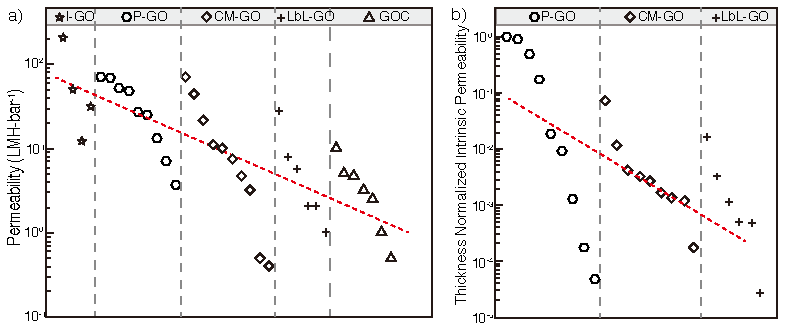
\includegraphics[width=5in]{paper3/Fig2.pdf}
  \caption{\textbf{GO chemistry I.} \textbf{(a)}  Photo of the six GO samples in solution (left). A color gradient relative to the O/C ratio (right). \textbf{(b)} C1s spectra obtained by XPS analysis of GO samples. The data also display the percentage contribution of individual peaks obtained by deconvolution and the O/C ratio.}
  \label{Fig2_pap3}
\end{figure}

As seen in Fig.~\ref{Fig2_pap3}, XPS quantitatively characterizes the chemistry of GO thin films with limited and automated post-processing of the data (\textit{e.g.}, C1s peak deconvolution), leading to high-throughput measurements. The chemistry of GO thin films was also analyzed with spectroscopic techniques such as, UV-vis, ATR-IR, and Raman spectroscopy Fig.~\ref{Fig3_pap3}a. From the UV-vis spectra for Samples $2-6$ in Fig.~\ref{Fig3_pap3}a, it is possible to observe an absorbance peak around 220 nm representing the $\pi-\pi^*$ transition of the aromatic C=C bonds remaining from the original graphitic structure.\cite{paredes2008graphene} In contrast, Sample 1 is characterized by a red-shifted peak ($\approx230$ nm) due to its lower oxidation state,\cite{li2014waveband} confirming a lower oxygen content compared to the other samples. Furthermore, Sample 1 also presents multiple shoulder peaks (blue rectangle in the inset zoom) related to multilayer GO structures,\cite{lai2012ultraviolet} where the carbon planes can approach one another closely enough to allow $\pi-\pi^*$ stacking, which also leads to a broader absorption peak in the region around 600 nm. Although the XPS analysis indicated that Samples $2-6$ are characterized by a wide-range of oxidation states ($0.43<$O/C$<0.55$), the UV-vis fails to convey this information.

\begin{figure}[t!]
  \centering
  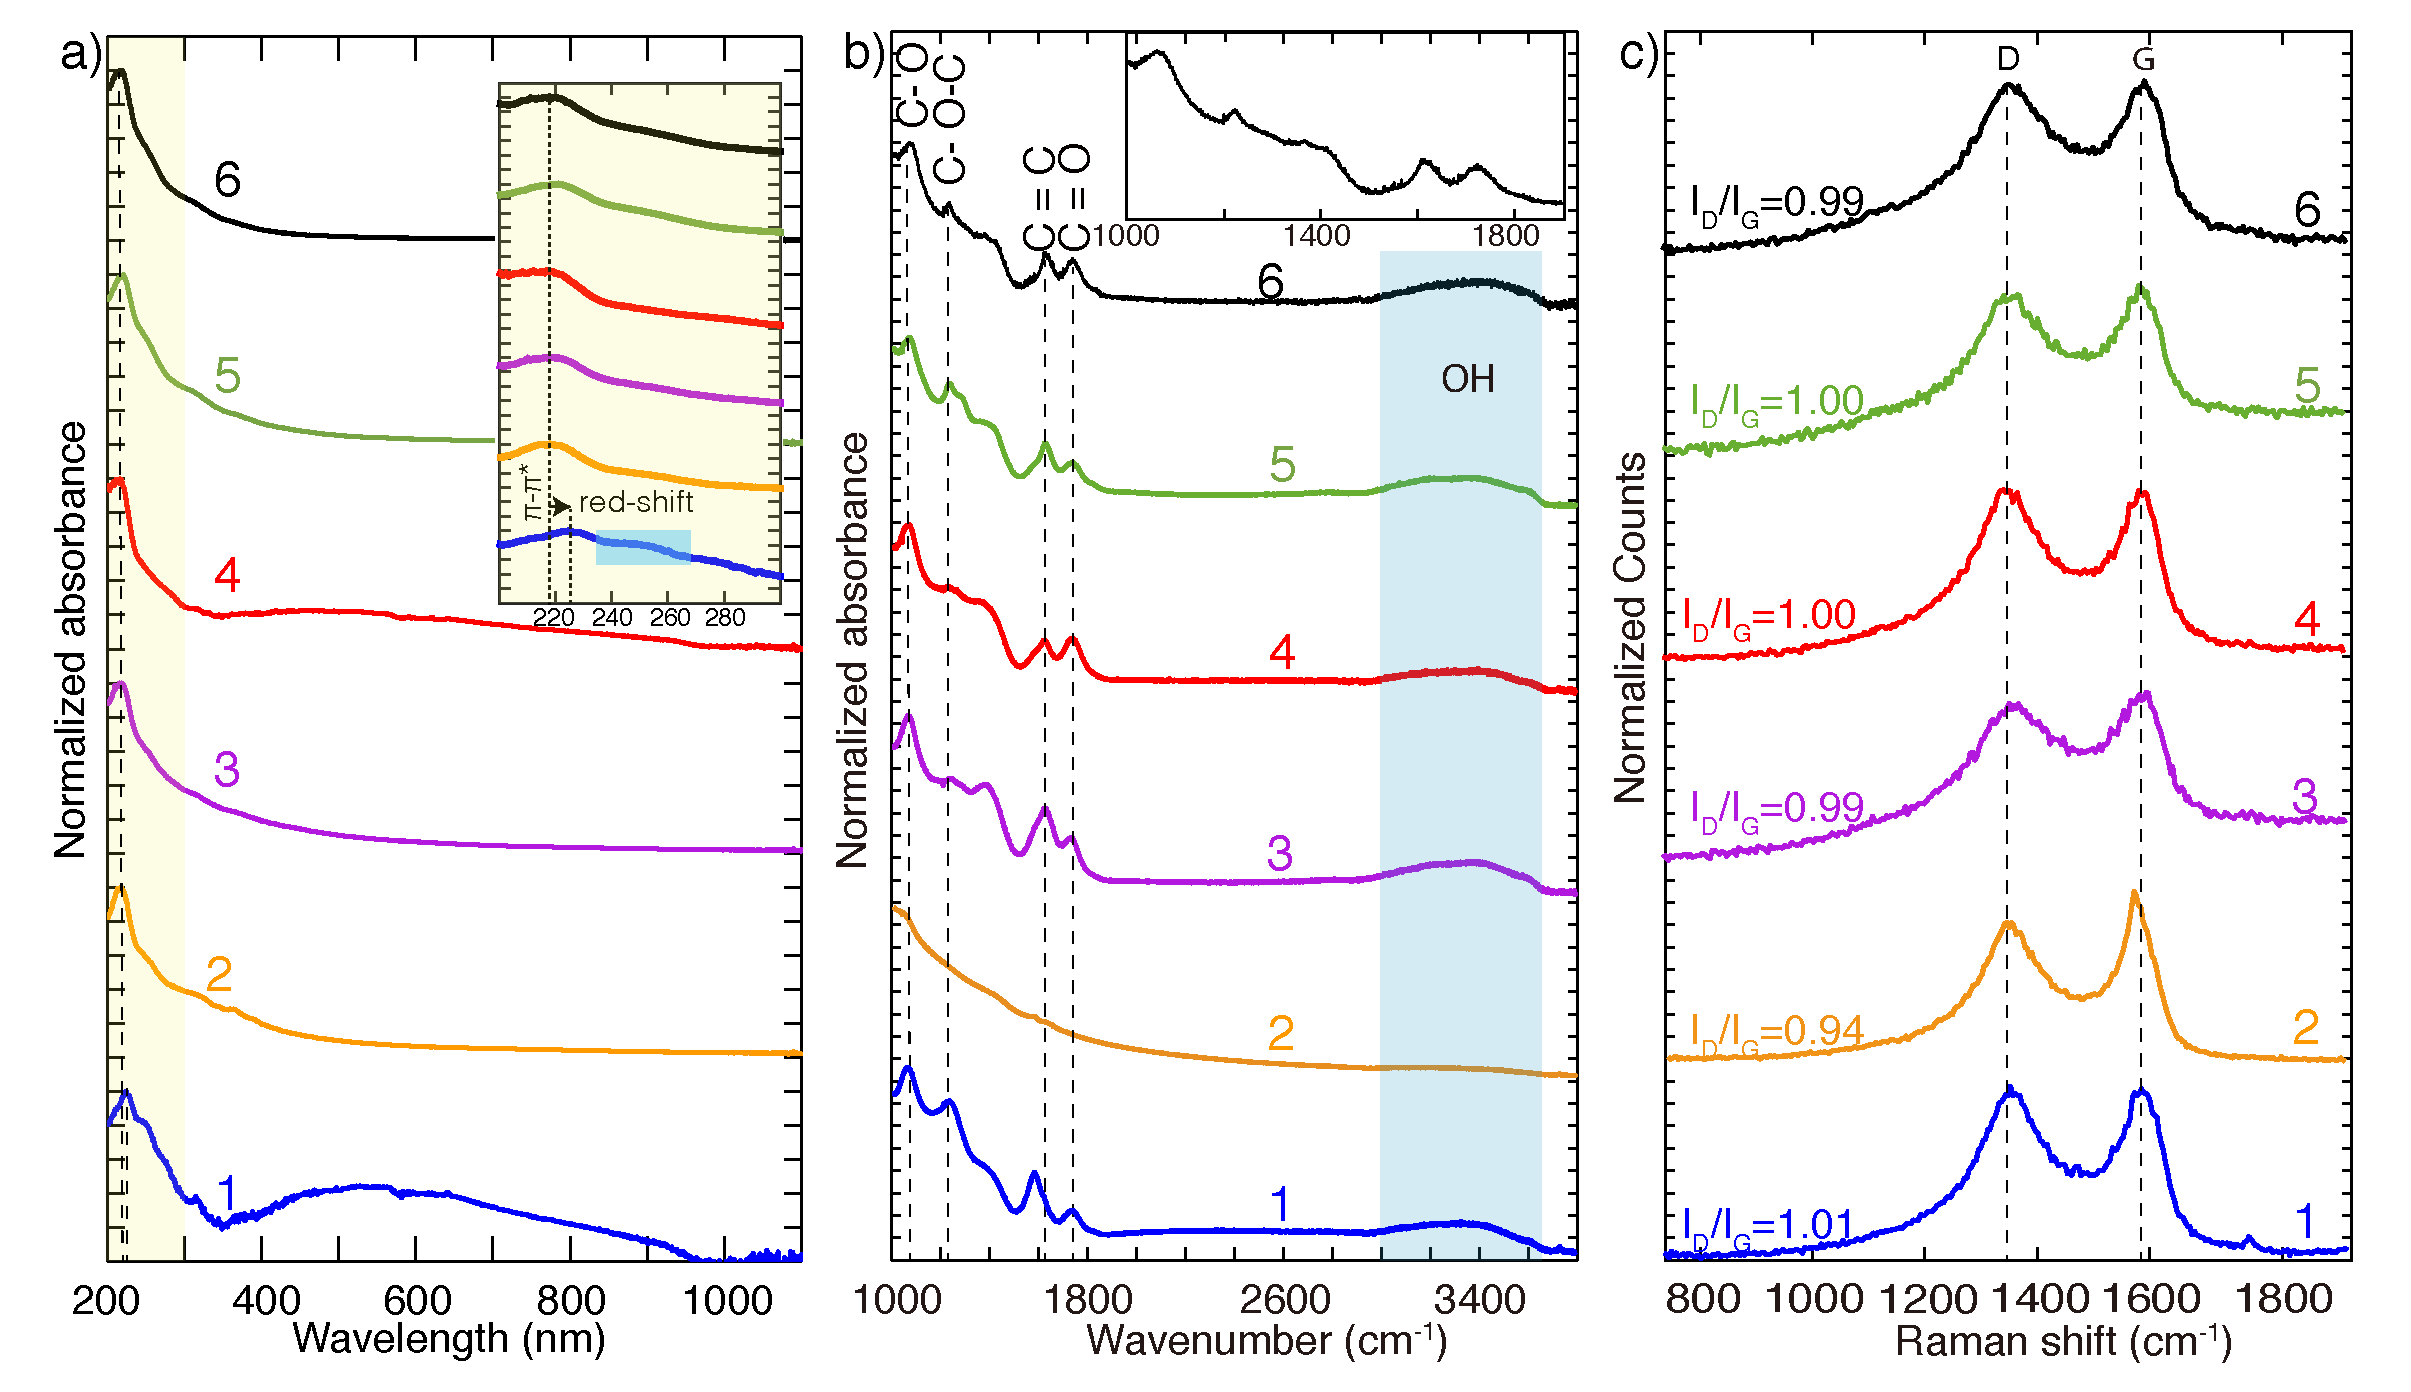
\includegraphics[width=6in]{paper3/Fig3.pdf}
  \caption{\textbf{GO chemistry II.} \textbf{(a)}  UV-vis, \textbf{(b)} ATR-IR, \textbf{(c)} ATR-IR, Raman spectra of the six GO samples.}
  \label{Fig3_pap3}
\end{figure}

In Fig.~\ref{Fig3_pap3}b, the IR spectra confirms the oxidation of GO with alkoxyl, epoxide, and carboxylate peaks centered at 1065, 1230, and 1730 cm\textsuperscript{-1}, respectively.\cite{xia2015ultrathin} The other major peak centered at 1625 cm\textsuperscript{1} is due to the presence of sp\textsuperscript{2} domains. The IR also displays a broad absorbance spectrum in the region $3200-3600$ cm\textsuperscript{-1} related to OH stretching vibrations of adsorbed water for all the samples except for Sample 2 (\textit{i.e.}, the sample with no XPS carboxylate peaks). Although IR spectroscopy is able to quantify the concentration of gases via the Lambert-Beer law, the quantification of the thin film materials' functionalities is challenging. The IR spectrum can be strongly influenced by the calibration curve, the morphology of the sample, and, in the case of ATR, also by the area of contact between the material and the germanium crystal. Thus, it is difficult to quantitatively compare the chemistry of different samples and the user can only report qualitative functionality information based on the presence or absence of peaks or relative change over time of a single sample. In summary, UV-vis and IR spectroscopy are useful techniques for confirming the GO oxidation state and identify functionalities, but are not able to quantify GO chemistry and oxy-functionalities since spectra from different samples are indistinguishable.\\
Raman spectra have also been used by researchers to characterize GO;\cite{yang2009chemical} in our case, the six Raman spectra samples are presented in Fig.~\ref{Fig3_pap3}c, and display a D-band at $\approx1350$ cm\textsuperscript{-1}, representative of defects/disorder in the basal plane, and a G-band at $\approx1590$ cm\textsuperscript{-1} representative of the in-plane sp\textsuperscript{2} bond stretching.\cite{amadei2016increase} A primary quantifiable Raman measurement is the D/G intensity ratio (I\textsubscript{D}/I\textsubscript{G}), which is a measurement of the defect density. However, all GO samples with different XPS oxidation states display I\textsubscript{D}/I\textsubscript{G}$\approx1$, apart from Sample 2 which has a slightly lower defect density I\textsubscript{D}/I\textsubscript{G}$\approx0.94$); thus, Raman is not a suitable technique for quantifying the GO chemistry. Moreover, Raman spectroscopy tends to be a destructive technique\cite{rogala2016observer} for a metastable material such as GO; even a short laser irradiation time ($<2$ s) would be sufficient to alter GO chemo-morphological structure and is likely responsible for the lack of Raman variation with oxidation state. In addition, during GO reduction, CO and CO\textsubscript{2} are liberated producing defects; thus, one cannot reliably characterize partially reduced GO samples with Raman because the reduction converts one type of defect (oxy-groups) to another type (vacancies) produced during reductive deoxygenation.\\
Zeta Potential (ZP) can also be used to indirectly analyze the chemistry of materials in aqueous solutions. The ZP of moderately stable GO dispersions (ZP $\leq-30$ mV) in water at pH$\approx7$ is summarized in Table~\ref{tbl1_pap3}. The negative charge is connected to the ionization of the carboxylate functional groups, again indicating successful GO oxidation\cite{li2008processable} and making aqueous GO dispersion stable from aggregation. For Sample 1, it was not possible to obtain reproducible ZP values, since the material was not stable to aggregation and sedimentation in water. As observed by XPS, Sample 1 is characterized by the lowest extent of oxidation, which does not provide sufficient electrostatic repulsion to stabilize the colloidal solution, resulting in aggregation and subsequent settling of the GO dispersion (see Fig.~\ref{figS2_AppA} in the Appendix A).\\
Static contact angle (SCA) provides information on the properties of a thin film, such as the GO chemistry, assuming that the morphology of GO film does not significantly vary (\textit{i.e.}, all thin films here are made with the same casting procedure). The SCA decreases from $\approx60$\textdegree\ to $\approx25$\textdegree\ with increasing oxidation state (from Sample 1 to Sample 6). This result is related to a higher affinity of water to more highly oxidized surfaces, due to the increase in hydrophilicity, in accordance with previous reports analyzing the wettability of GO in different oxidation states.\cite{li2014tuning} In particular, the presence of hydrophilic functional groups (\textit{e.g.}, hydroxyl) decreases the hydrophobic nature of pristine graphene and increases its surface energy. As stated for the UV-vis and IR techniques in Fig. 3, although ZP and SCA can deliver useful qualitative information on the GO oxidation state, this information cannot be directly translated into quantifiable properties across samples.
\begin{table}[ht]
 \begin{center}
 \caption{\textbf{Zeta potential (ZP), static contact angle (SCA), and Z-Avg for the six GO samples.}}
  \label{tbl1_pap3}
  \begin{tabular}{cccc}
        \hline
        Sample & ZP (mV) & SCA (\textdegree) & Z-Avg (nm)\\
        \hline
        1 & n/a           & $60.5\pm2.1$   & n/a\\
        2 & $-38.1\pm1.4$ & $ 49.3\pm1.7$  & $596\pm14$\\
        3 & $-32.4\pm1.1$ & $39.3\pm3.3$   & $1981\pm224$\\
        4 & $-33.2\pm0.3$ & $29.7\pm1.7$   & $507\pm134$\\
        5 & $-38.1\pm1.4$ & $25.7\pm1.7$   & $1503\pm32$\\
        6 & $-29.7\pm1.7$ & $25.3\pm2.3$   & $1604\pm21$\\
        \hline
  \end{tabular}
 \end{center}
\end{table}
\subsection{Graphene Oxide Morphology}
After analyzing the GO chemistry, the attention is turned to techniques for characterizing GO flake morphology. SEM images and statistical data obtained by image processing are presented in Fig.~\ref{Fig4_pap3}.
A representative SEM image for each of the samples is dis- played in Fig.~\ref{Fig4_pap3}a, whereas the statistical data in Fig.~\ref{Fig4_pap3}b-c is based on multiple images (see Methods). SEM image data analysis was used to quantify the flake size distribution (see ~\ref{Fig4_pap3}b and Fig.~\ref{figS1_AppA} in the Appendix A for details). In Fig.~\ref{Fig4_pap3}b, the flake areas have log-normal distributions (dashed red lines) characterized by a few larger flakes and more numerous smaller flakes. Noteworthy is the great extent of the variability of the average GO flake area between samples, which spans over an order of magnitude (\textit{e.g.}, from 0.2 to 9.3 $\mu$m\textsuperscript{2}). In particular, Samples 3, 5, and 6 are characterized by larger GO flakes than those in Samples 1, 2 and 4. This difference is also captured by Z-Avg hydrodynamic diameter measurements, which are $>1500$ nm and $<600$ nm for Samples (3, 5, 6) and (2, 4), respectively (Table~\ref{tbl1_pap3}). In the case of GO, Z-Avg measurements cannot be compared to the actual flake size measured by other techniques since they are assumed to be monodispersed samples with spherical or near-spherical shape (GO is 2D) that uniformly scatter light (GO is partially transparent).\cite{xiong2016ultrarobust,zhao2010efficient} For Sample 1, it was not possible to obtain a hydrodynamic value, since it is characterized by a polydispersivity index of 1 indicating that the sample likely contains aggregates that can sediment leading to a skewed size distribution (Fig.~\ref{figS2_AppA}). In SEM images, GO flakes in the same image are characterized by different greyscale intensities: monolayer flakes appear brighter compared to multilayer aggregates. Using this intensity difference, we are able to quantify the percentage of monolayer for each sample (see Fig.~\ref{figS3_AppA} for details).\cite{amadei2016increase} GO Samples $2-6$ have a monolayer percentage $>78$\% confirming effective exfoliation and the 2D nature of GO. For Sample 1, SEM analysis confirms UV-vis and Z-Avg results, which indicated the presence of multilayer structures and large aggregates as only 15\% of the flakes are monolayer and the intensity distribution displays multiple peaks related to flakes with various numbers of GO layers (\textit{e.g.}, multilayer).\\
\begin{figure}
  \centering
  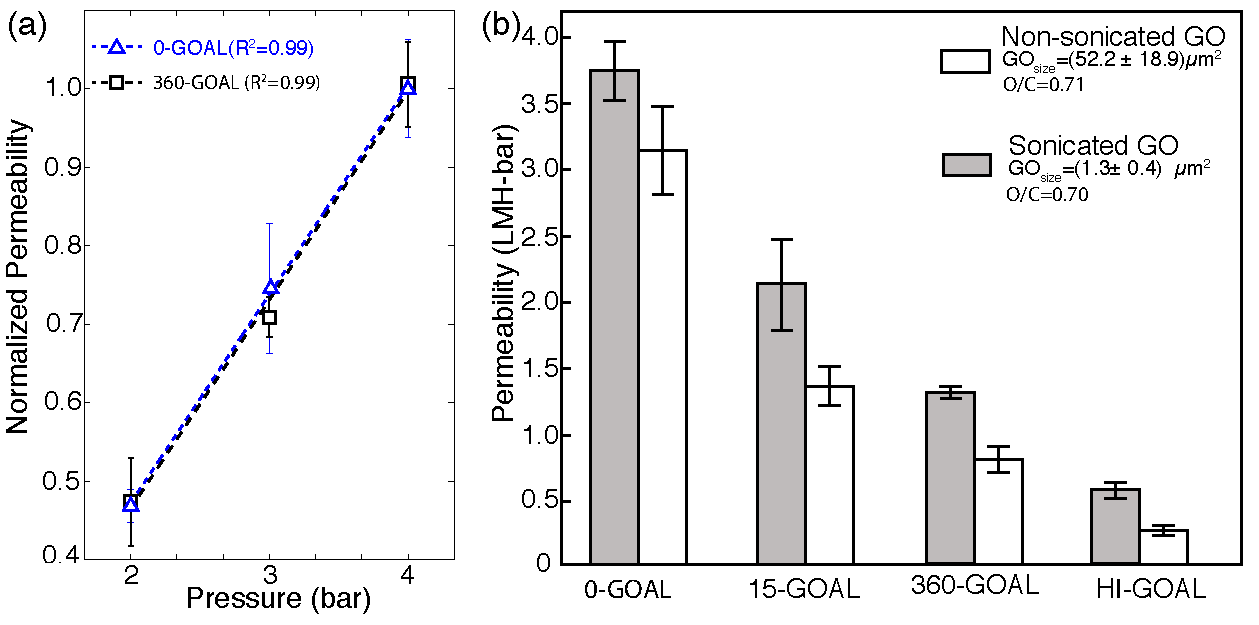
\includegraphics[width=4.5in]{paper3/Fig4.pdf}
  \caption{\textbf{GO morphology I.} \textbf{(a)} SEM images of GO samples. \textbf{(b)} GO flake size distribution fitted to a log-normal distribution (red dashed lines); yellow square represents zoom in for the smaller GO flakes (Samples 1, 2, and 4). \textbf{(c)} Histograms of SEM image greyscale intensities that are deconvoluted to obtain mono-/multi-layer percentages.}
  \label{Fig4_pap3}
\end{figure}
Although SEM can quantify the percentage of monolayer structures and geometry of the GO flakes, the flake thickness is another important morphological parameter for a 2D material. XRD of a GO thin film is able to measure the separation distance ($2h$) between GO flakes due to GO's tendency to stack in a laminar fashion. XRD can give an approximation of the combined GO thickness including intercalants, such as water molecules, which will remain unless specific and rigorous drying protocols are used. The GO separation distance varies $\approx15$\% from Sample 1 to Sample 6 (from 7.9 to 9.1 {\AA}) increasing with increasing GO oxidation and basal plane oxy-functionality (Fig.~\ref{Fig5_pap3}a). Thereby, GO samples with higher extent of oxidation result in a less compacted thin film structure, whereas GO samples with lower extent of oxidation result in a more compacted thin film structure. Moreover, under ambient conditions GO samples with higher extent of oxidation will absorb more water molecules than the ones with lesser extent of oxidation. Considering that the graphene layer itself has a known vdW thickness of 0.34 nm and addition of oxygen groups can increase that thickness to $6-7$ {\AA}, any GO with a thickness larger than that is influenced by water adsorption. GO thickness can also be measured via AFM, however, AFM measurements can vary depending on the mode of operation and environmental conditions. As an example, GO morphology for Sample 5 obtained by operating the AFM in non-contact mode\cite{san2002unifying} (attractive regime, phase values above 90\textdegree) is displayed in Fig.~\ref{Fig5_pap3}b. The GO monolayer thickness is $\approx2$ nm, which is considerably higher than the 1.5 nm thickness evaluated in contact mode\cite{san2002unifying} (Fig.~\ref{Fig5_pap3}c, repulsive regime, phase values below 90\textdegree). Both values are in accordance with previously reported GO thickness.\cite{stankovich2007synthesis} AFM results may also be affected by the AFM tip geometry and ambient conditions (\textit{e.g.}, presence of humidity),\cite{santos2012effects} which will increase the thickness of the water layer trapped between the substrate and the GO flakes.\cite{santos2012method} For this reason, AFM images comparing GO flakes from different producers are not presented here. However, AFM is useful for corroborating the monolayer nature of the GO observed by SEM.\\

\begin{figure}
  \centering
  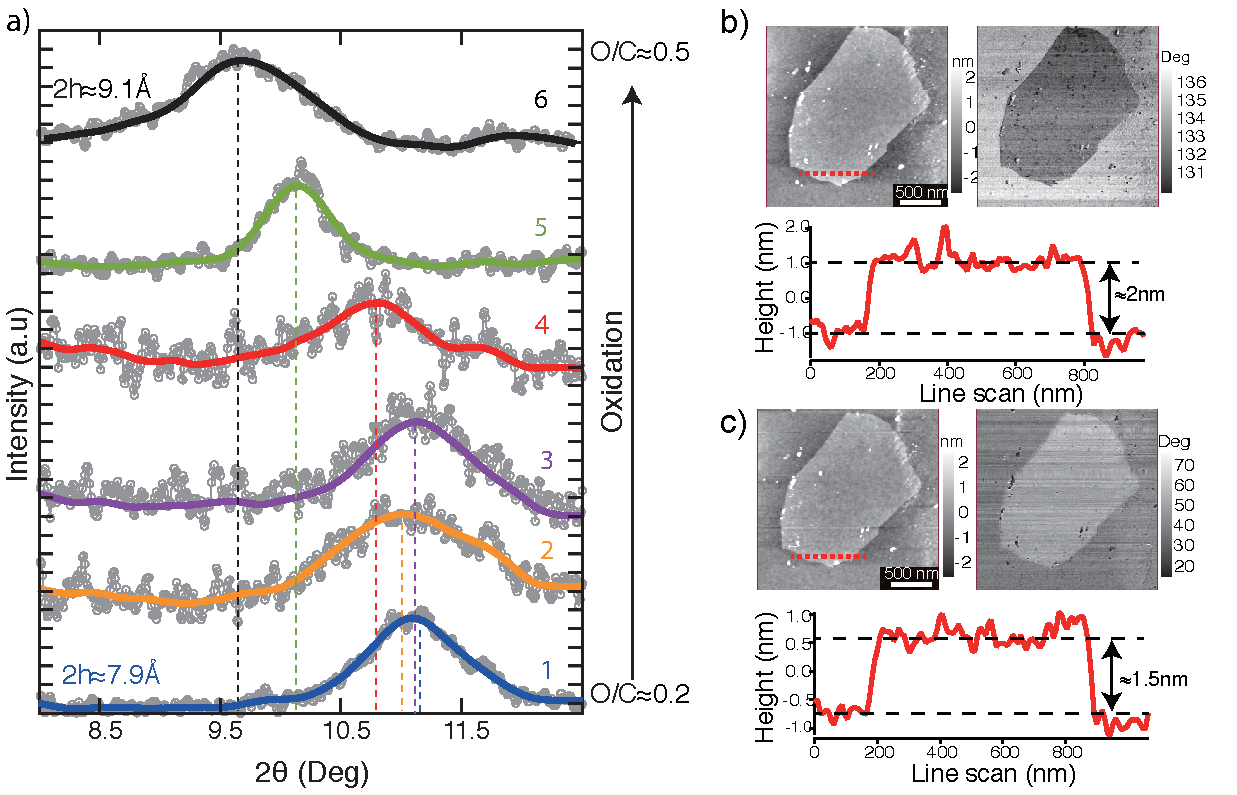
\includegraphics[width=4in]{paper3/Fig5.pdf}
  \caption{\textbf{GO morphology II.} \textbf{(a)} XRD spectra for the six GO samples. AFM analysis in  \textbf{(b)} non-contact attractive and \textbf{(c)} contact repulsive regime for a single GO flake.}
  \label{Fig5_pap3}
\end{figure}

\subsection{Graphene Oxide Characterization Tools}
All the tools used in this study to characterize the chemistry and morphology of GO are classified in Table~\ref{tbl2_pap3}. The information provided by the different techniques is divided between quantitative and qualitative; the latter should only be used in the GO prescreening phase and/or to obtain results in relative (and not absolute) terms that could validate quantitative measurements. To summarize, XPS is the primary tool to quantitatively analyze GO chemistry due to the ability to provide information regarding the oxidation state and the specific GO oxy-functionalities with minimal and automated data post-processing. Disregarding the time needed to pump down the XPS (pump and instrument dependent), an XPS measurement generally takes $1-2$ min per sample. On the other hand, SEM is the primary tool to quantitatively characterize the GO morphology providing information on the monolayer nature and on the dimensions of the GO flakes. For SEM, the image acquisition generally takes $1-2$ min per sample. Thus, the time required to quantitatively characterized the chemo-morphological GO properties is quite attractive. Other microscopy techniques, such as TEM or STEM, have not been included in this study as they would convey similar data obtained already by SEM on the GO morphology. However, TEM and STEM can give information regarding the atomic structure of GO\cite{dave2016chemistry} and the interaction between GO and other nanostructures, such as metal nanoparticles.\cite{shao2015preparation} In regard to XRD, researchers can infer information on both chemistry and morphology from the separation distance $2h$, with a characterization time on the order of minutes per sample depending on the number of spectra acquired; moreover, XRD does not require particular experimental conditions. The alternative techniques presented here such as ATR-FTIR, UV-vis, and Raman spectroscopy can deliver complimentary qualitative information on GO morphology and chemistry, which can be used for prescreening or as orthogonal measurements.
\begin{sidewaystable}
 \begin{center}
 \caption{\textbf{Summary of the techniques used to characterize the GO chemistry and morphology.} In bold are highlighted the quantitative techniques.}
  \label{tbl2_pap3}
  \begin{tabular}{cccc}
        \hline
        Technique & Morphology & Chemistry & Notes\\
        \hline
        XPS & - & \textbf{Quantitative} & O/C atomic and oxy-functional group ratios via C1s peak deconvolution\\
        Color Chart & - & Qualitative & Related to oxidation state\\
        UV-vis & Qualitative & Qualitative & Presence/extent of sp\textsuperscript{2} conjugation and multilayer nature/structure\\
        ATR-IR & - & Qualitative & Presence of specific oxy-functional groups and sp\textsuperscript{2} conjugation\\
        Raman & -  & Qualitative & Defect and sp\textsuperscript{2} conjugation, but destructive to sample\\
        SCA & -  & Qualitative & Wettability as indirect measure of oxidation and surface roughness\\
        ZP & - & Qualitative & Surface charge as indirect measure of oxidation (deprotonated oxy-groups)\\
        SEM & \textbf{Quantitative} & -  & Flake size distribution and monolayer percentage via image analysis \\
        XRD & \textbf{Quantitative} & Qualitative  & Flake-to-flake separation influenced by the presence of oxy-groups \\
        AFM & Semi-Quantitative & -  & GO thickness highly sensitive to experimental and operation conditions\\
        Z-Avg & Semi-Quantitative & -  & Hydrodynamic flake size distribution, skewed by spherical/opaque assumptions\\
        \hline
  \end{tabular}
 \end{center}
\end{sidewaystable}
\subsection{Graphene Oxide Standardization}
Careful research of the GO literature ($>300$ peer-reviewed articles) was carried out in order to collect information on the chemistry and morphology of GO used in previous studies. The O/C atomic ratio distribution for GO, reduced GO (RGO), and multilayer (\textit{i.e.}, nanoplatets) GO (MLGO) found in the literature are presented in Fig.~\ref{Fig6_pap3}a. 

\begin{figure}[h]
  \centering
  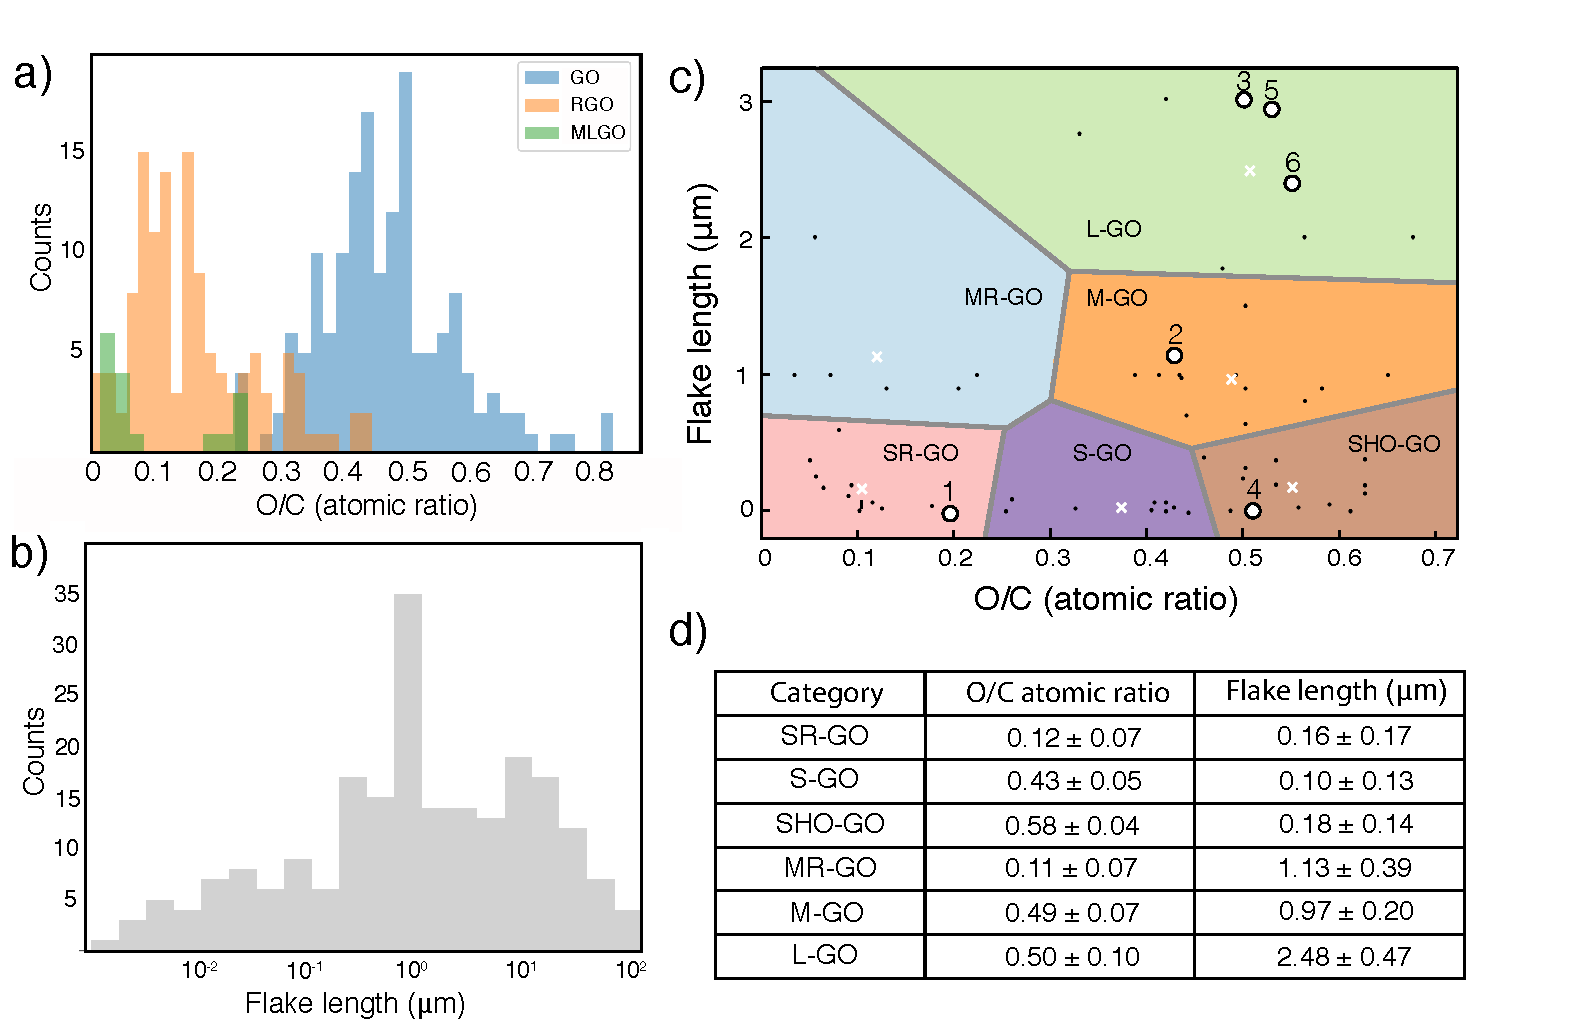
\includegraphics[width=6in]{paper3/Fig6.pdf}
  \caption{\textbf{GO characterization in the literature.} \textbf{(a-b)} O/C atomic ratio and mean flake size distribution histograms. Each count represents a scientific work. \textbf{(c)} K-mean classification of the GO characterization based on O/C atomic ratio and mean flake size. Every white ''x'' represents the centroid (mean) of each class, white circles represent GO samples used in this study, and black dots represent the chemo-morphological data obtained from literature review.  \textbf{(d)} The table lists the nanoscopic properties for the centroid of each category; the mean flake size of the samples used in this study was calculated from areas in Fig.~\ref{Fig4_pap3}b assuming a square GO flake.}
  \label{Fig6_pap3}
\end{figure}

The distribution greatly varies as the O/C atomic ratio for GO and RGO are characterized by very different average values, $0.46\pm0.13$ and $0.16\pm0.10$, respectively. MLGO has an O/C similar to RGO due to its poor exfoliation. The variation in the dimension of the GO flake is even greater than the O/C atomic ratio and spans over five orders of magnitude as illustrated in Fig.~\ref{Fig6_pap3}b. This variation is caused by the significant difference in the dimension of the starting materials (\textit{i.e.}, graphite flakes)\cite{zhao2010efficient} and/or processes such as sonication and centrifugation used during GO synthesis and post-processing.\cite{amadei2016fabrication,Goncalves2014,khan2012size,lin2012fabrication} The large variation in the nanoscopic GO properties hinders a true comparison among scientific works and can generate confusion in the research community. For this reason, an initial attempt to statistically classify GO based on its chemo-morphological properties is presented in Fig.~\ref{Fig6_pap3}c. The majority of the GO literature was researched in order to locate scientific works that characterized both GO chemistry and morphology and the data was classified using the K-mean clustering algorithm.\cite{bishop2006pattern} The basic idea behind K-mean clustering is to determine the minimum number of classes into which the data will be partitioned, and then perform computations to group data so that observations within a cluster are similar and observations in different clusters are dissimilar. Each cluster is characterized by a centroid, which is typically the mean of the data. The algorithm assigns each observation to one cluster randomly and then repeats the following two steps until the clusters do not change: i) for each cluster computes the centroid; ii) given the centroids, reassigns all the observation based on their closeness to centroids. Via this iterative process, a local minimum is found by minimizing a cost function (details in Methods). K-mean clustering classified the chemo-morphological data (black dots) into six categories: small and less oxidized GO (SLO-GO in pink), small GO (S-GO, in purple), small and highly oxidized GO (SHO-GO, in brown), medium and less oxidized GO (MLO-GO, in blue), medium GO (M-GO, in orange), and large GO (L-GO, in green). By assuming a Gaussian distribution of data points, the centroid (white exes in Fig.~\ref{Fig6_pap3}c) of each cluster is characterized by an O/C atomic ratio and a mean flake size as presented in the table in Fig.~\ref{Fig6_pap3}d. According to this characterization, Sample 1 is classified as SLO-GO, Sample 2 as M-GO, Sample 4 as SHO-GO, and Samples 3, 5 and 6 as L-GO. The fact that three samples felt in the same category could be an indication of a predominant GO synthesis method in industry, which yield nanomaterials with the same property. Note that the classification presented here can be refined with the introduction of data from future peer-reviewed publications. However, this classification could be used by producers to properly advertise their material and by researchers in presenting their work to allow for a more reliable comparison of results between different studies, and ultimately facilitating the rational development of GO-based applications.
Furthermore, the 2D material chemo-morphological properties might have a significant impact on the industrial device performance. For this reason, we investigated a number of GO-based applications with GO material from different producers. In particular, we focused on applications that are relevant to the use of GO in membrane separation processes, which has recently attracted the attention of many research groups.\cite{mi2014graphene,willcox2017molecular,huang2015graphene} The fabrication process (\textit{e.g.}, quantity of GO used in membranes and casting technique) was the same for all the membranes, and the tests were conducted by the same researcher reducing output variability related to experimental procedure. Thus, it is assumed that the variability in the results is primarily related to different GO properties.\\
The first application evaluated was bacterial adhesion onto GO membranes (GOM), which was motivated by recent reports indicating intrinsic antifouling properties of GOM in water treatment applications (\textit{e.g.}, nanofiltration, forward osmosis, etc.).\cite{hegab2015fine,hu2014layer} The bacterial adhesion results are summarized in Fig.~\ref{Fig7_pap3}a and Table~\ref{tbl3_pap3}. GOM were immersed in a solution containing bacteria (\textit{E. coli}) for 20h (see Methods) and the extent of bacterial deposition on the membrane surface was evaluated via SEM analysis. The variation in bacterial deposition behavior (bacterial adhesion $\approx50$\% and $>75$\%) is highlighted by comparison of SEM for Sample 6 (L-GO,  Fig.~\ref{Fig7_pap3}a top) and Sample 4 (SHO-GO, Fig.~\ref{Fig7_pap3}a bottom). Representative images for the other samples can be found in Fig.~\ref{figS4_AppA}. By comparing images in Fig.~\ref{Fig7_pap3}a, it is observed that larger GO flakes (Sample 6) result in increased deposition of \textit{E. coli} as recently reported.\cite{perreault2015antimicrobial} This trend was also observed for the other samples (see Table~\ref{tbl3_pap3}) in which GOM composed of L-GO lead to higher ($1.5-2$-fold higher) bacterial adhesion. The variation is likely connected to the higher number of intrinsic defects of smaller flakes that hinders bacterial adhesion. For example, it has been reported that the presence of higher defect surface density in small flakes as compared to large flakes will induce oxidative stress and reduce bacterial adhesion.\cite{perreault2015antimicrobial}

\begin{figure}
  \centering
  \includegraphics[width=6in]{paper3/Fig7.pdf}
  \caption{\textbf{Performance comparison of GO toward macroscopic applications.} \textbf{(a)} Representative SEM images of \textit{E. coli} bacteria adhesion onto GOM (Samples 6 and 4, top and bottom image, respectively).  \textbf{(b)} MB adsorption of GO samples before (top) and after (bottom) centrifugation.  \textbf{(c)} Permeability data of GOM at 5 bar (top) and schematic of their GO flake arrangement (bottom).}
  \label{Fig7_pap3}
\end{figure}

\begin{table}[t!]
 \caption{\textbf{Performance GO-based applications samples in terms of bacterial adhesion, adsorption properties, and permeability.}}
  \label{tbl3_pap3}
  \begin{tabular}{ccccc}
        \hline
        Sample & Category & Bacterial Adhesion & Adsorption &  Permeability\\
        & & (bacteria/area)\textsuperscript{*} & (MB removal, LRV)& (10\textsuperscript{3} LMH-bar)\\
        \hline
        1 & SLO-GO & $46\pm10$  & $1.11\pm0.17$  & $38.3\pm16.8$\\
        2 & M-GO   & $53\pm22$  & $1.48\pm0.17$  & $0.5\pm0.5$\\
        3 & L-GO   & $77\pm215$  & $1.55\pm0.17$ & $128.4\pm73.8$\\
        4 & SHO-GO & $51\pm10$  & $1.44\pm0.17$  & $186.3\pm59.8$\\
        5 & L-GO   & $100\pm28$  & $1.46\pm0.16$ &  $116.9\pm69.6$\\
        6 & L-GO   & $75\pm12$   & $1.45\pm0.15$ &   $171.6\pm71.6$\\
        \hline
  \end{tabular}
      \small
      \item\textsuperscript{*} Data have been normalized to 100 to increase readability. 100 bacteria/unit corresponds to 75 bacteria per 7000 $\mu$m\textsuperscript{2}.
\end{table}
The second application was the use of GO for the adsorption of methylene blue (MB), which is often used as a representative molecule for cationic dye wastewater. The adsorption of organic molecules is a fundamental parameter to evaluate when calculating the rejection properties of a filter or membrane. The introduction of MB in most GO solutions causes an instantaneous aggregation of GO flakes (Fig.~\ref{Fig7_pap3}b  top) due to GO surface charge neutralization.\cite{yang2011removal,li2013comparative} The GO MB aggregation phenomenon occurs in all samples, apart from Sample 1. The MB solution was in contact with the GO for 24 h, then the solution was centrifuged and the supernatant was extracted (Fig.~\ref{Fig7_pap3}b  bottom) to quantify the MB removal via UV-vis (see methods section for further details). The GO MB adsorption capacities are compared via the log removal value (LRV) and summarized in Table~\ref{tbl3_pap3}. All GO samples have an average MB log removal capacity between 1.44 and 1.55 except for Sample 1 (SLO-GO), which has a log removal capacity of $\approx1$. Although Samples 4 and 1 are similarly characterized by small flakes, Sample 4 (SHO-GO) displays a 27\% higher removal capacity compared to Sample 1 (SLO-GO); thus, the adsorption capacity cannot be connected to morphology. MB adsorption is more related to the GO surface charge due to the presence of oxy-functional groups\cite{krishnamoorthy2013chemical,ramesha2011graphene} \textit{i.e.}, the lesser number of oxy-functional groups for Sample 1 (O/C atomic ratio $<0.2$ as compared to $0.43-0.55$ for Samples $2-6$) results in a lesser MB adsorption capacity.\\
Although membrane permeability is a primary parameter in the design of membrane systems, recent studies report GOM permeabilities ranging over orders of magnitude.\cite{amadei2016increase} The GOM permeability for the six different samples obtained by capillary flow porometry is displayed in Fig.~\ref{Fig7_pap3}c top and Table~\ref{tbl3_pap3}. A large variation in the permeability (up to a factor of five) is observed, which is related to the variation in GO chemistry and morphology between samples. As recently proposed, GOM permeability is affected by two primary factors:\cite{amadei2017role} i) flake size, which is proportional to membrane pore tortuosity, thus inversely proportional to permeability; and ii) extent of oxidation, which is directly proportional to the width of GO nanochannels or interlayer separation distance (XRD data in Fig.~\ref{Fig5_pap3}a), thus permeability. In summary, both GO chemistry and morphology will affect the GOM membrane permeability and a scheme illustrating the individual effects of these two factors is displayed in Fig.~\ref{Fig7_pap3}c bottom. Samples 3 and 5 have similar oxidation and flake size, leading to similar permeability results. Sample 4 displays the highest permeability value, predominantly due to both its high O/C ratio value (high nanochannels width) and small flake size (low tortuosity). Although Samples 4 and 6 exhibit similar permeability results, the cause is significantly different; for Sample 4 the permeability is partially originated by a small flake size (reduced tortuosity), whereas for Sample 6 the permeability is mostly driven by the increased O/C ratio (increased width of GO interlayer nanochannels), which compensates the larger flake size. Sample 1 displays a significant lower permeability due to the poor oxidation of the GO flakes leading to narrow GO nanochannels. Incorporation of GO into polymer membranes has been reported to enhance permeability by increasing overall membrane hydrophilicity.\cite{zinadini2014preparation} Similarly, here the most hydrophilic GOM samples (SCA$<40$\textdegree) have a higher permeability. In contrast, Sample 2 was nearly impermeable under 5 bar of applied pressure due to the absence of carboxylate functional groups (Fig.~\ref{Fig2_pap3}b), which creates a compacted laminate structure and reduces wettability as corroborated by the absence of an O-H water vibration band in Fig.~\ref{Fig3_pap3}b.
\section{Conclusions}
By defining the most relevant characterization techniques, a vast-range of GO materials were classified into distinct categories according to their chemo-morphological properties. The classification process is based on GO chemistry and morphology determined by SEM image analysis and XPS spectra analysis. A K-mean clustering algorithm classified the chemo-morphological data into six categories SLO-GO, S-GO, SHO-GO, MLO-GO, M-GO, and L-GO. Although the classification relied on thorough literature research ($>300$ papers) for calibration, this work does not represent an ultimate classification process and could be extended and refined with other characterization techniques and more training data (\textit{e.g.}, future research investigations). The main goal of this work is to create momentum and raise awareness about the need of a GO standardization process and that the existing variation in device performance obtained from different research groups may be attributed to the highly variable properties of the GO starting material. This was highlighted in the last part of this work, in which GO-based applications yielded quite different results based on the diversity of what should have been, as advertised, the ''same'' GO material. This initial GO classification aims to facilitate the recognition of adequate material by setting standards for industrial GO producers. Concurrently, researchers will be able to make fair comparisons and increase the reproducibility of their and interlab results, leading to a higher signal to noise ratio in the development of GO materials for practical applications.





